\section{Design of the system [VI]}

The system consists of three main components: data source, data processing, and data storage.
Figure~\ref{fig:SpeedLayerArchitecture} depicts the general structure of the system.

\begin{figure}[h]
  \centering
  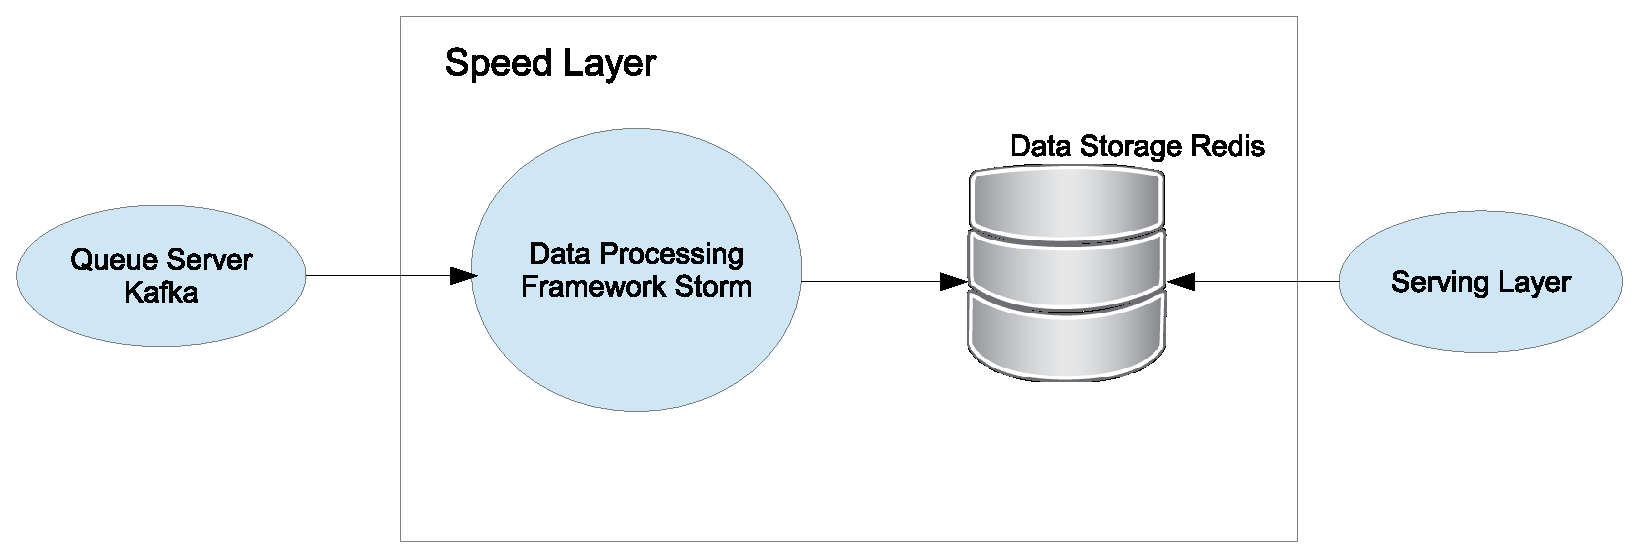
\includegraphics [width=1.0\textwidth]{images/SpeedLayerArchitecture}
  \caption{General structure of the Speed Layer.}
  \label{fig:SpeedLayerArchitecture}
\end{figure}

The source of the system is a queue server Kafka \ref{subs:kafka}.
It receives data from the outer sources, specifically from smartphones.
It stores them temporarily, and tries to send them to all consumers, until they acknowledge delivery.
Our system is one of the consumers, and when it receives a message, it starts its processing. 

The data processing framework Storm \ref{subs:storm} is the main component of the system.
It receives messages from Kafka queue server, and performs different computations on that data.
Its purpose is to provide different aggregatons on data coming from smartphones.
These aggregations are then stored in the storage system, and can be accessed by the Speed layer for answering queries.

Data storage Redis \ref{subs:redis} is a place, where all results of computations are kept.
These results are different aggregations, specifically counters, that are stored in the complex data model.
Redis provides simple access to save and then get that data.
Counters, saved in the Redis data storage can be then used by the Speed layer to merge them with the results of batch computations.

\subsection{Data source}

Originally data comes from tens of thousends of smartphones.
Their number can grow arbitrarily, what requires in essence to have such a complex distributed server.
Smartphones send data to the server in small batches, that contain about several tens of events, that happened since the last sending.
The server receives events and puts them to the Kafka queue server, that tries then to transmit them to consumers.
One of consumers is the Kafka spout, that is the part of the data processing topology, that we build in Storm.

Kafka provides 

topics and spouts for each event type

\subsection{Data processing}
storm
topology
bolts
events
aggragations
anomaly detection
classes

\subsection{Data storage}
redis
keys
access to redis
transactions and pipelining